%!TEX root = ../thesis.tex

\section{ ARCHITECTURE }
\subsection{ Client }

The first significant part of the application is the client which will
be the interface for the user to manipulate map and data. The core functionality of the client
is follows:

\begin{enumerate}
  \item Panning and zooming map.
  \item Selecting a point on the map to build a whole graph of
  the routes needed to move from selected point to all other points of the city. All of the routes
  are parametrized by color and width. These parameters are calculated utilizing information
  about transport type specified in this point and the coefficient which is defined as number of
  times this particular line is used in all of the directions calculated from this point.
  \item Showing prevailing transport in all points of the grid. Prevailing transport is defined
  by calculating total time spent in each transport type. The maximum of all of the values will
  be taken as prevailing.
  \item Showing fastest and slowest roads. The map should also have interactive slider
  which will be used to filter roads within particular speed range.
  \item Showing most accessible points on the grid. The transport accessibility coefficient of the
  point can be defined as total time spent in a transport while moving from selected point to all
  other points. All of the values after that scaled to be between 0 and 1. This view should also
  have a filter by transport accessibility coefficient.
\end{enumerate}

For the reason of the easy distribution it was selected to use browser based client. Thus
client is implemented as single-page web application, which should support all modern browsers such
as Safari, Google Chrome, Firefox, Microsoft Edge.

\subsection{ RESTful Server }

For serving data to the client it was selected to utilize RESTful~\cite{rest:wiki} architectural
style, which represents HTTP approach to read, update and delete data. Due to the fact, that our
application will only read data and not modify it, then we will only need to describe all of
the end-points for data access where data will be encoded in GeoJSON~\cite{geojson:spec}.
For our application following end-points were selected:

\begin{itemize}
  \item \textbf{\texttt{GET /points}} \\
  The returned points are described as FeatureCollection of points with following
  properties (see also Listing~\ref{lst:points_format}):

  \begin{description}
    \item[name] is a string;
    \item[id] is a unique identifier of the point encoded as string;
    \item[prevalingTransport] could be \mbox{``BUS''}, \mbox{``TROLLEYBUS''},
    \mbox{``TRAM''}, \\ \mbox{``SUBWAY''}, \mbox{``COMMUTER\_TRAIN''}, \mbox{``SHARE\_TAXI''},
    \mbox{``DRIVING''}, \\ \mbox{``WALKING''}.
    \item[accessibility] is a floating number in range from 0 to 1.
  \end{description}

  \begin{lstlisting}[language=json, caption=Points response example, label=lst:points_format]
  {
    "type": "FeatureCollection",
    "features": [
      "type": "Feature",
      "geometry": [0,0],
      "properties": {
        "id": 0,
        "name": "Location Name",
        "prevailingTransport": "SUBWAY",
        "accessibility": 0.6
      }
    ]
  }
  \end{lstlisting}

  \item \textbf{\texttt{GET /lines?point\_id}}

  This endpoint is parametrized by point\_id which means that if point id is presented
  then the client will receive only those lines which are associated with specified point.
  On the other hand, if no point id is not specified all lines are returned.

  The properties of the lines can be describe as follows (see also Listing~\ref{lst:lines_format}):
  \begin{description}
    \item[id] is a unique identifier of the line encoded as string;
    \item[travelMode] is on of the \mbox{``BUS''}, \mbox{``TROLLEYBUS''},
    \mbox{``TRAM''}, \\ \mbox{``SUBWAY''}, \mbox{``COMMUTER\_TRAIN''}, \mbox{``SHARE\_TAXI''},
    \mbox{``DRIVING''}, or \\ \mbox{``WALKING''}.
    \item[weight] number of times this line was used in all of the routes across all of
    the directions' set.
    \item[duration] time needed to travel this line in seconds.
    \item[distance] total length of this line in meters.
  \end{description}

\begin{lstlisting}[language=json, caption=Lines response example, label={lst:lines_format}]
{
  "type": "FeatureCollection",
  "features": [
    "type": "Feature",
    "geometry": [[0,0], [0,0]],
    "properties": {
      "id": 0,
      "width": 1,
      "weight": 200
      "duration": 100,
      "distance": 400,
      "travelMode": "BUS"
    ]
  }
}
\end{lstlisting}
\end{itemize}

It is important to note that we could also add such filtering parameters as \texttt{speed} and
\texttt{travelMode}, but it was revealed during set of experiments that
filtering on server side can take significant amount of time which is up to few
hundreds seconds. Hence, this parameters were dropped and filtering is performed on the client.

Suggested architecture implies that client will perform rendering using GeoJSON data, although
it was investigated that for our purposes rendering becomes rather slow and after series of
optimizations the best rendering time was close to 3 seconds. The next improvement to the
current scheme will be adding tile server which can significantly speed up rendering time.

\subsection{ Tile Server }
Graphical map tiles are usually rectangular images in raster or vector format. Most of the popular
map library providers utilize tiles~\cite{google:tiles, mapbox:tiles} for rendering their maps.
Raster tiles are basically images which do not allow to change color of roads and landscapes.
In contrast, vector tiles are not just images but structures which contain geometries and
metadata such as roads, rivers, places in special compact format. Vector tiles only rendered when
requested by the client.

There are several benefits of using vector tiles. The first, advantage is small size of the tiles,
which allows rendering of high resolution and caching. The second advantage is an ability to change
style of the layers: adjust colors of the geometry, line width, set borders to polygons,
set background patterns. Finally, maps based on vector tiles allow smooth transitions between
zoom levels. Although, the cost of usage of the vector tiles is the lack of
compatibility with older browsers. At the moment most of the libraries demand WebGL support and
latest browser versions which are Chrome 49.0, Safari 9, Internet Explorer 10 and higher,
Microsoft Edge 13~\cite{google:support,mapbox:support}. Another drawback of usage tiles is
that geometry can not be transformed in real-time and rendering small amounts of data is actually
slower than GeoJSON approach.

Switching from GeoJSON server to vector-tile server resulted in considerable speed improvement.
If previously rendering time took around 3 seconds and amount of transfered data was around 1.8 Mb,
then with tile server rendering takes less than a second and size of the data transfered to the
client is around 100 kb.


\subsection{ Summary }

Although, tiles suit well for rendering considerable amounts data, for points rendering it was
decided to utilize GeoJSON data. The final architecture is illustrated on
Figure~\ref{pic:architecture} and can be described as follows:

\begin{enumerate}
  \item Web-based client supporting latest browsers.
  \item GeoJSON RESTfull server providing points data.
  \item Tile server providing data about lines.
\end{enumerate}

\begin{figure}[t]
  \centering
  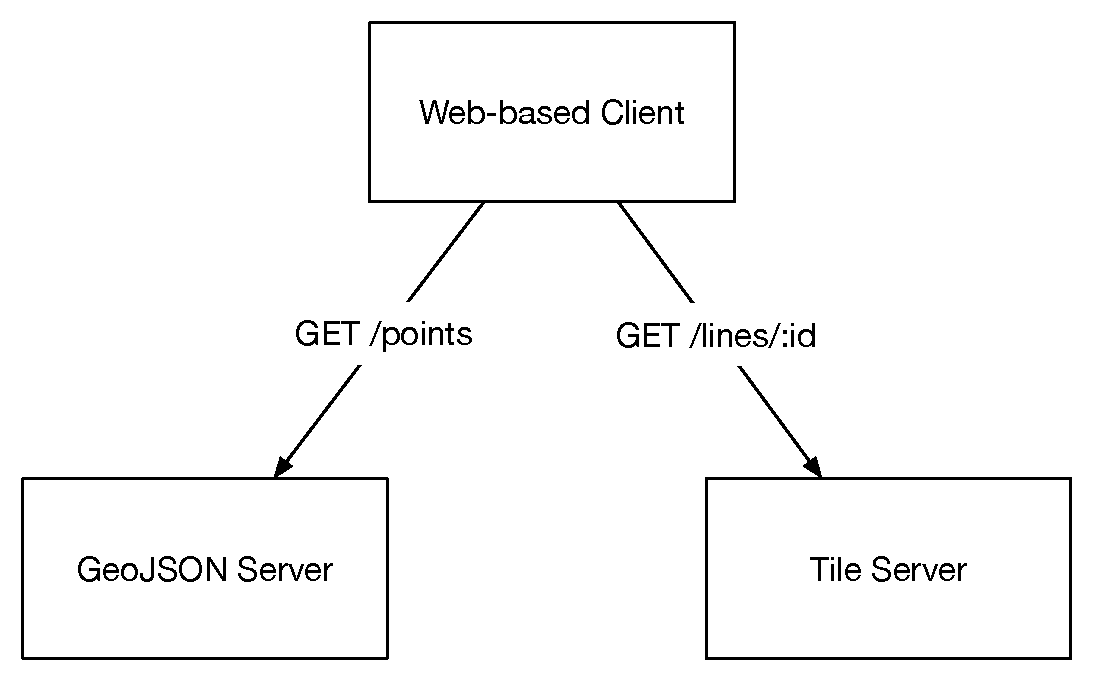
\includegraphics[width=0.7\textwidth]{architecture.pdf}
  \caption{Final system architecture.}
  \label{pic:architecture}
\end{figure}
